\documentclass[tikz]{standalone}
\usepackage{tikz}
\usetikzlibrary{intersections,calc,quotes,angles}
\usepackage{tkz-euclide}
\begin{document}

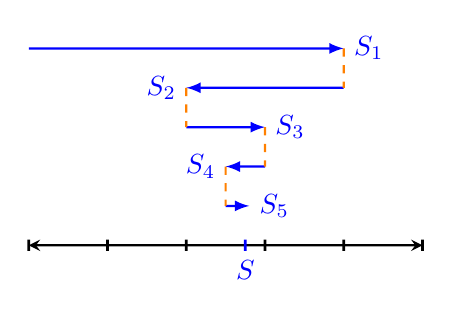
\begin{tikzpicture}[transparency group=knockout]

  \draw[<->, > = stealth, thick] (0, 0) -- (5, 0); 
  \draw[-latex,color=blue,thick](0,2.5) -- (4,2.5) node[right] {$S_1$};
  \draw[-latex,color=blue,thick](4,2.0) -- (2,2.0) node[left] {$S_2$};
  \draw[-latex,color=blue,thick](2,1.5) -- (3,1.5) node[right] {$S_3$};
  \draw[-latex,color=blue,thick](3,1.0) -- (2.5,1.0) node[left] {$S_4$};
  \draw[-latex,color=blue,thick](2.5,.5) -- (2.8,.5) node[right] {$S_5$};
  \draw[-,dashed,color=orange,thick] (4,2.5) -- (4,2);
  \draw[-,dashed,color=orange,thick] (2,2) -- (2,1.5);
  \draw[-,dashed,color=orange,thick] (3,1.5) -- (3,1);
  \draw[-,dashed,color=orange,thick] (2.5,1) -- (2.5,.5);
  \draw[blue] (2.75,2pt) -- (2.75,-2pt) node[below] {$S$};
  \foreach \x in {0, 1, ..., 5} {\draw (\x, 2pt)--(\x, -2pt);};
\end{tikzpicture}
\end{document}